\section{METODOLOGI}

Penelitian ini dilaksanakan sesuai dengan blok diagram pada Gambar 3.1. Blok diagram tersebut
merupakan metodologi penelitian yang disusun sesuai dengan langkah-langkah yang dilakukan dalam penelitian ini.

\begin{figure} [ht] \centering
  \counterwithin{figure}{section}
  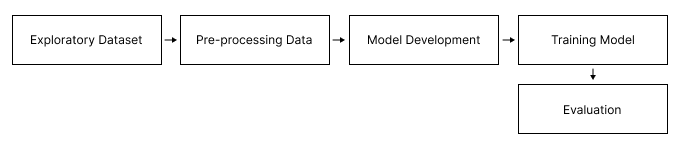
\includegraphics[width=160mm]{gambar/metodologi.png}
  \caption{Metodologi Penelitian}
\end{figure}


\subsection{Exploratory Dataset}
\lipsum[14]

\subsection{Pre-processing Data}
\lipsum[14]

\subsection{Training}
\lipsum[14]

\subsection{Evaluation}
\lipsum[14]

\subsection{Recommend}
\lipsum[14]

